
\chapter{概述}
\section{交通信号概述}
交通信号控制是一个重要而具有挑战性的现实问题,其目的是通过协调车辆在道路交叉口的运动来最小化所有车辆的通行时间。目前广泛使用的交通信号控制系统仍然严重依赖过于简化的信息和基于规则的方法。车联网技术的发展、硬件性能的提升以及人工智能技术的进步使得我们现在有更丰富的数据,更多的计算能力和先进的方法来驱动智能交通的发展。 
交通信号控制的目的为了方便车辆在交叉路口的安全和高效移动。安全是通过信号灯指定不同车道的车通行来分离相互冲突的运动实现的。为了能够有效地优化通行效率,已有的工作提出了不同的指标来量化通行效率,主要有以下三个:
1.	通行时间:在交通信号控制中,车辆的行驶时间被定义为一辆汽车进入系统的时间与离开系统的时间的差值。 最常见的优化目标之一是就是减少进过路口的所有车辆的平均通行时间。
2.	队列长度:队列长度是指路口等待车辆的数量,越大的队列长度意味着越多的等待车辆,路口的通行效率越低,反之通行效率越高。
3.	路口吞吐量:吞吐量是指在一定期间内进过路口完成通行的车辆数量。越大的吞吐量代表着越高的通行效率,所以很多工作将最大化吞吐量作为优化的目标。
\section{基本术语}
Approach: 指交叉路口的巷道。任何一个交叉路口都有两种approach,进入路口的incoming approach和离开路口的outgoing approach。图3.a描述了一个典型的有8个approach(四个入口,四个出口)的交叉路口。
Lane: 一个Approach是由一组车道组成。与Approach的定义类似,车道也分为两种:转入车道(incoming lane)和转出车道(outgoing lane)。
Traffic movement:指的是车流从一个incoming approach 运动到另一个outgoing approach,表示为 ,其中ri和ro分别表示incoming lane和outgoing lane。通常,traffic movement可以分为左转、直行以及右转三种,在少数特殊的路口也支持U-turn的traffic movement。
Movement signal:根据traffic movement定义的运动信号,绿色代表可以通行,红色代表禁止通行。根据大多数国家的交通规则,右转的traffic movement是可以不受信号约束的。
Phase: 信号灯的一个phase(相位)是指非冲突运动信号的组合,这意味着这些信号可以同时设置为绿色,而不会引起安全冲突。 图3.c展示了最常用的四相位信号模式。
Phase sequence: 相序,即一组相位的序列,它定义了一组相位及其变化顺序。
Signal plan:信号计划,由一组相位序列及其相应的起始时间组成。通常表示为 其中 和 分别代表相位及其开始时间。
Cycle-based signal plan:周期性信号计划,与普通的信号计划不同的是其中的相位序列是按循环顺序工作的,可以表示为 其中 是重复出现的相位序列, 是j周期中相位pi的起始时间。具体地, 是第j周期的周期长度, 是第j周期中的相位分裂比(phase split ratio),表示每个相位持续时间占总周期长度的比重。现有的交通信号控制方法通常在一天中重复类似的相位序列。

\section{传统交通控制方法}
\subsection{Webster}
对于单个交叉口,交通运输工程领域中的交通信号控制方法通常由三个部分组成:确定信号周期长度,确定信号相位序列以及相位分裂。Webster是一种广泛使用的计算单个交叉路口的信号周期长度和相位分裂时间的方法。通过假设车流在一段时间内(例如,过去的五分钟或10分钟)是均匀到达的,可以计算出确切的最优周期和最佳相位分裂时间,从而最小化车量通行时间。

\subsection{GreenWave}
虽然使用Webster可以简单的控制单个交叉路口的交通信号,但是对于相邻的多个交叉路口,不能够简单地直接使用Webster来分别优化每一个路口,相邻路口信号灯的信号时间之间的偏移(即相邻路口信号周期起始时间的差值)也需要进行优化,因为对于相距较近的路口来说,一个路口的控制策略可能会影响到其他路口。
GreenWave就是交通运输领域中最经典的协调相邻路口的信号控制方法,它通过优化相邻路口信号时间的偏移来减少车辆在某一方向行驶时的停留次数。这种方法可以形成沿指定交通方向的绿色信号波,在该方向行驶的车辆可以受益于渐进的绿色信号级联,而不会在任何交叉口停留,如下图所示:
\begin{figure}[htb]
    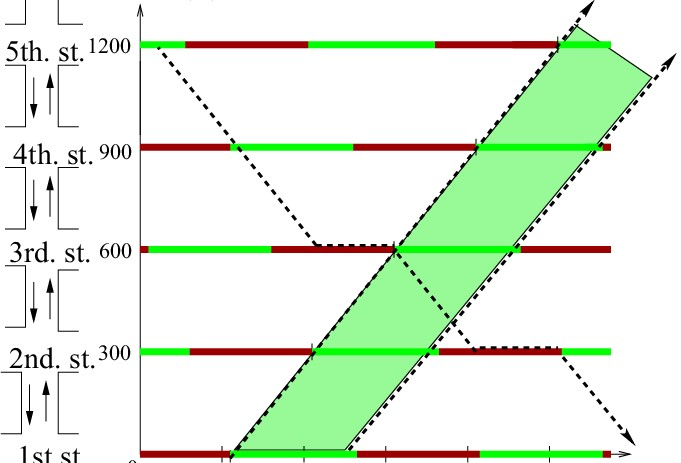
\includegraphics[width=10cm]{fig/GreenWave.jpg}
    \caption{路口敏感性说明}
    \label{fig:green-wave}
\end{figure}

\subsection{Actuated Control}
Actuated Control根据当前相位和其他的竞争相位对绿色信号的请求来决定是否保持或者变化当前的相位。请求规则如下:
1. 当目前相位的持续时间未达到最小时间周期时,或在当前相位对应入车道上有车辆进入,并且在接近信号的距离内时,就会产生延长绿色信号时间的请求,已让车辆可以直接通过路口。 
2. 当竞争相位的等待车辆数量大于一个阈值时,就会生成对绿色信号的请求。
根据规则的差异,Actuated Control主要可以分为Fully-Actuated Control和Semi-Actuated Control两种。

\subsection{SOTL}
Self-Organizing Traffic Light Control(SOTL)是一种具有附加需求响应规则的Fully-Actuated Control方法。它与Fully-Actuated Control的主要区别在于当前相位的绿色信号请求定义(虽然它们都需要最小的绿色相位持续时间):在Fully-Actuated Control中,当车辆接近信号灯时,就会产生延长绿色信号的请求,而在SOTL中,除非接近信号灯的车辆数量大于不一定是一个阈值,否则就不会产生请求。

\subsection{Max-Pressure Control}
Max-Pressure Control的目的是通过最小化对应相位的压力(pressure)来平衡相邻路口之间的队列长度,从而降低过饱和的风险,其中压力的概念如下图所示:
\begin{figure}[htb]
    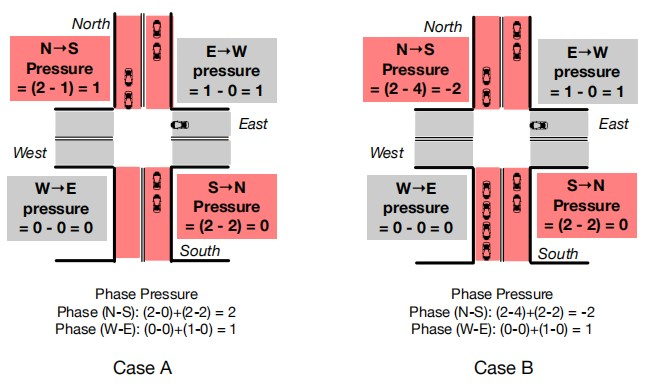
\includegraphics[width=10cm]{fig/max-pressure.jpg}
    \caption{路口敏感性说明}
    \label{fig:max-pressure}
\end{figure}
从形式来看,运动信号的压力可以定义为(交通运动的)传入车道上的车辆数减去相应的传出车道上的车辆数;相位的压力定义为传入通道和传出通道上的总队列长度之间的差异。Varaiya等人证明了当将优化目标设为最小化单个路口的相位压力时,Max-Pressure Control可以最大限度地提高真个路网的吞吐量。

下表列出了每种方法的限制和要求:
\begin{table}[htb]
    \caption[协作策略]{常见的协作策略\label{tab:coordination}}
    \begin{tabular}{llll}
      \toprule
      方法 & 先验信息 & 输入 & 输出 \\
      \midrule
      Webster & 相位序列 & 交通流量 & 基于周期的单个路口信号计划 \\
      GreenWave & 信号计划 & 交通流量、速度限制、车道长度 & 基于周期的信号计划的偏移量 \\
      Actual Control, SOTL & 相位序列& 交通流量 & 是否变化到下一个相位\\
      Max-Pressure Control & 无 & 队列长度 & 所有交叉口的信号计划\\
      \bottomrule
    \end{tabular}
\end{table}

\section{基于强化学习的交通信号控制}
最近,人们提出了不同的人工智能技术来控制交通信号,例如遗传算法、群体智能以及强化学习。 其中在这些技术中,强化学习在近年来更具趋势。
\subsection{强化学习概述}
通常单智能体强化学习问题被建模成MDP $<\mathcal{S}, \mathcal{A}, P, R, \gamma>$,其中$\mathcal{S}, \mathcal{A}, P, R, \gamma$分别表示状态集、动作集、概率状态转移函数、奖励函数和折扣因子。具体定义如下:
\begin{itemize}
    \item $\mathcal{S}$:在时间步骤$t$,智能体得到一个观测状态$s^t \in \mathcal{S}$。
    \item $\mathcal{A}, P$:在时间步骤$t$,智能体采取一个动作$a^t \in \mathcal{A}$,然后环境根据状态转移函数转移到一个新的状态。
    \begin{align}
        P\left(\mathrm{~s}^{t+1} \mid \mathrm{s}^{t}, \mathrm{a}^{t}\right): \mathcal{S} \times \mathcal{A} \rightarrow \mathcal{S}
    \end{align}
    \item $R$:在时间步骤$t$,智能体通过奖励函数获得一个奖励$r^t$。
    \begin{align}
        R\left(s^{t}, a^{t}\right): \mathcal{S} \times \mathcal{A} \rightarrow \mathbb{R}
    \end{align}
    \item $\gamma$:智能体的目标是找到一种使预期收益最大化的政策,即折扣奖励之和。折扣因子决定了即时奖励与未来奖励的重要性。
    \begin{align}
        G^{t}:=\sum_{i=0}^{\infty} \gamma^{i} r^{t+i}
    \end{align}
  \end{itemize}
\subsection{基于强化学习交通信号控制框架}

\subsection{基本要素}
使用强化学习来解决交通信号控制问题要先确定以下几个基本要素:

奖励设计:由于强化学习是以最大化累计奖励为目标来学习的,所以奖励的选择决定了学习的方向。在交通信号控制问题中,虽然最终目标是尽量减少所有车辆的通行时间,但由于几个原因,通行时间很难直接作为RL的有效奖励。首先,车辆的行驶时间不仅受交通信号灯的影响,还受车辆自由流动速度等其他因素的影响。其次,当交通信号控制器事先不知道车辆行驶目的地(在现实世界中往往是这样),优化道路上所有车辆的通行时间变得特别困难。 在这种情况下,车辆的通行时间只能在多个动作完成后车辆完全离开路口后才能测量。已有工作的奖励设计通常是基于一些可以直接在一个动作后测量的指标的加权和。例如,等待车辆的队列长度、车辆等待时间、速度、累计延迟、路口的吞吐量、车辆平均停车次数、信号变化频率(信号在一定时间段内变化的次数,学习到的策略不应该太过频繁的改变信号)以及路口的压力(Max-pressure中定义的pressure)等。虽然将奖励定义为几个因素的加权线性组合是现有研究中的一种常见做法,并且取得了不错的效果,但是这种特别的设计存在两个问题。第一,无法保证最大化设计的奖励等价于最优的通行效率,因为它们在交通运输理论中没有直接联系。第二,调整每个奖励函数因子的权重是相当棘手的,在权重设置上的微小差异可能会导致最终的结果有显著的差别。
状态表示:状态表示是以一种数值化的形式来描述路口的交通状况,描述的越全面越有利于学习到最优策略,通常使用多个要素组合来描述交通状况,例如,队列长度、车辆等待时间、车辆数量(包含非等待车辆),车辆速度、车辆位置分布以及当前信号灯的相位等。最近,在基于RL的交通信号控制算法中出现了使用更复杂状态的趋势,希望能够更全面地描述交通状况。 Mousavi、Van derPol以及Wei Hua等人在他们的研究工作中提出使用位置图片来当作状态描述。但是,具有如此高维度的状态学习往往需要大量的训练样本,这意味着训练RL代理需要很长时间。 更重要的是,较长的学习进度不一定会导致显著的性能增益,因为代理可能有更困难的时间从状态表示中提取有用的信息。因此,状态的表示应该简洁且能够充分地描述环境。
动作选择机制:动作选择机制决定了以何种方式来控制信号灯,不同的动作机制有不同的影响。主要可以总结为以下四种方式:
\begin{itemize}
    \item 确定当前相位时长:在这中动作选择机制下,智能体学习通过从预定义的候选时间段(比如,10秒、15秒、20秒等)中选择来设置当前相位的持续时间。
    \item 确定基于周期的相位比:这种方式定义的动作为下一个周期的相位分裂比(phase split ratio) 通常,给出总周期长度,并预先定义一个包含一些相位比的候选集。
    \item 保持或改变当前相位:这种方式也是基于周期性的信号计划,通常一个二进制数来定义动作。例如,1表示保持当前相位,0表示变换到下一相位。
    \item 选择下一个相位:这种方式直接从待选相位序列中选择一个相位并变化到该相位,其中相位序列不是预定的。因此,这种信号控制方式更加的灵活,智能体学习在不同的而状态下选择最优的相位,而不假设信号会以循环的方式改变。
\end{itemize}
学习算法:
协作策略:
